\documentclass[a4paper]{article}
\usepackage[affil-it]{authblk}
\usepackage[english]{babel}
\usepackage[backend=bibtex,style=numeric]{biblatex}

\usepackage{geometry}
\geometry{margin=1.5cm, vmargin={0pt,1cm}}
\setlength{\topmargin}{-1cm}
\setlength{\paperheight}{29.7cm}
\setlength{\textheight}{25.3cm}

% useful packages.
\usepackage{amsfonts}
\usepackage{amsmath}
\usepackage{amssymb}
\usepackage{amsthm}     
\usepackage{abstract}
\usepackage{booktabs}
\usepackage{enumerate} %enumerate environment
\usepackage{graphicx}
\usepackage{multicol}
\usepackage{fancyhdr}
\usepackage{url}
\usepackage{multirow}
\usepackage{amsfonts}
\usepackage{mathrsfs}
\usepackage{upgreek}
\usepackage{caption}
\usepackage{subcaption}
\usepackage{layout}
\usepackage{ctex}      %中文环境
\usepackage{booktabs}  %三线表
\usepackage{verbatim}  %comment environment
\usepackage{float}     %强制表格图片位置
\usepackage{listings}  %insert code in latex
\usepackage{fontspec}  %font support
\usepackage{tikz}
\usetikzlibrary{shapes, arrows}
\usepackage{makecell}
\usetikzlibrary{intersections}
\usepackage{arydshln}


\usepackage[colorlinks,linkcolor=blue]{hyperref}
\usepackage{xcolor}
\definecolor{mygreen}{rgb}{0,0.6,0}
\definecolor{lightgrey}{rgb}{0.95,0.95,0.95}
\definecolor{winered}{rgb}{0.5,0,0}
\definecolor{mymauve}{rgb}{0.58,0,0.82}
\lstset{
      backgroundcolor=\color{lightgrey},
      basicstyle             = \ttfamily,
      breakatwhitespace      = false,
      breaklines             = true,
      captionpos             = none,
      commentstyle           = \color{mygreen}\bfseries,
      extendedchars          = false,
      keepspaces             = true,
      keywordstyle           = \color{winered},         % keyword style
      language               = C++,                     % the language of code
      otherkeywords          = {string},
      numberstyle            = \tiny\color{mygray},
      rulecolor              = \color{black},
      showspaces             = false,
      showstringspaces       = false,
      showtabs               = false,
      stepnumber             = 1,
      stringstyle            = \color{mymauve},         % string literal style
      tabsize                = 2,
      title                  = \lstname,
      aboveskip              = 0pt,
      belowskip              = 0pt,
      columns                = flexible
}

% some common command
\newcommand{\dif}{\mathrm{d}}
\newcommand{\avg}[1]{\left\langle #1 \right\rangle}
\newcommand{\norm}[1]{\left\| #1 \right\|}
\newcommand{\difFrac}[2]{\frac{\dif #1}{\dif #2}}
\newcommand{\pdfFrac}[2]{\frac{\partial #1}{\partial #2}}
\newcommand{\OFL}{\mathrm{OFL}}
\newcommand{\UFL}{\mathrm{UFL}}
\newcommand{\fl}{\mathrm{fl}}
\newcommand{\op}{\odot}
\newcommand{\Eabs}{E_{\mathrm{abs}}}
\newcommand{\Erel}{E_{\mathrm{rel}}}
\addbibresource{citation.bib}


\begin{document}
% =================================================
\title{Book Report on "Statistical ranking and combinatorial Hodge theory"}

\author{Zhouyue Qian 3220104074
  \thanks{Electronic address: \texttt{3220104074@edu.zju.cn}}}
\affil{(Information and Computational Science Class 2201), Zhejiang University }


\date{Due time: \today}

\maketitle

\begin{abstract}
本读书报告针对现代电商与互联网场景中普遍存在的\textbf{不完整、不平衡基数数据},如Netflix评分、网页链接结构,,传统排名方法,如Kemeny优化,因计算复杂度高或数据兼容性不足而受限。本文引入\textbf{组合霍奇理论,Combinatorial Hodge Theory,},将排名问题转化为图论中的边流分解问题,通过离散外微积分与霍奇分解,将pairwise排名数据分解为\textbf{梯度流,全局一致排名,旋度流,局部循环不一致,和调和流,全局长程循环,}三部分。

核心方法包括:\\
\indent \textbf{图建模}:将待排名对象建模为图顶点,选民偏好转化为带权边流,构建pairwise comparison图,兼容基数评分、二元偏好等多类型数据。\\
\indent \textbf{霍奇分解}:利用组合梯度、旋度算子及图亥姆霍兹算子,Graph Helmholtzian,通过$l_2$投影分离数据的一致性与不一致性成分。其中,梯度流对应最小二乘意义下的最优全局排名,推广了传统Borda计数,旋度流量化三角循环矛盾,如Condorcet悖论,调和流刻画非三角的长程循环。\\
\indent \textbf{拓扑分析}:借助单纯复形,Simplicial Complexes,的贝蒂数,Betti Number,判断数据的全局一致性,例如一维贝蒂数为零表明局部一致蕴含全局一致。

通过Netflix电影排名、货币兑换市场、网页排名等实验,验证了HodgeRank在处理复杂数据时的有效性:
\indent  在Netflix数据中,通过旋度指标识别局部排名矛盾,如特定电影对的不一致偏好,,且对时间漂移具有鲁棒性；\\
\indent 在完整图场景,如货币市场,中,霍奇分解退化为无套利条件,证明理论一致性；\\
\indent 与PageRank相比,HodgeRank通过可逆马尔可夫链近似降低计算复杂度,适用于大规模网络。

本文的创新在于将拓扑学工具引入统计排名,为数据的多尺度分析提供了几何视角。HodgeRank不仅解决了传统方法在数据不完整场景的局限性,还通过\textbf{不一致性量化},如循环比率、相对旋度,为排名结果提供可靠性评估,为高维复杂数据的结构分析开辟了新路径。

\end{abstract}


% ============================================
\section{研究背景与问题}
\subsection{现代排名问题的兴起与数据特征}
作者开篇指出，排名问题在机器学习、电子商务、信息检索等领域日益重要。以Google搜索、Netflix推荐、eBay信誉系统为例，这类场景产生的\textbf{大规模数据集}呈现以下独特挑战：\\
\indent \textbf{数据类型的转变}：从传统的\textbf{序数排序}（如投票中的偏好顺序）转向\textbf{基数评分}（如1-5星评级），需保留评分差异的量化信息。\\
\indent \textbf{高度不完整性}：数据缺失普遍存在（如Netflix用户仅评价约0.1\%的电影），传统方法难以处理稀疏观测。\\
\indent \textbf{分布不平衡性}：热门对象（如畅销商品）的评分量远高于冷门对象，导致数据分布极度偏斜。\\
\indent \textbf{复杂网络结构}：数据隐含图结构（如网页超链接、用户-商品交互关系），需借助图论工具分析。

这些特征使得传统社会选择理论（如Condorcet、Borda方法）不再适用，迫切需要新的统计排名框架。\cite{Jiang2011StatisticalRanking}

\subsection{传统方法的局限性与新需求}
作者对比了传统排名方法的不足：\\
\indent \textbf{计算复杂度高}：Kemeny优化等方法需枚举排列组合，属于NP-hard问题，无法应对大规模数据。\\
\indent \textbf{数据兼容性不足}：假设数据完整且为序数类型，无法处理基数评分或缺失值。\\
\indent \textbf{缺乏结构分析}：仅输出单一排名，无法解释数据中的不一致性（如Condorcet悖论中的循环偏好）。

现代场景要求方法具备以下能力：\\
\indent 1.兼容基数与不完整数据：从稀疏评分中提取有效信息；\\
\indent 2.利用图结构：通过图论建模对象间的关联；\\
\indent 3.量化不一致性：区分局部矛盾与全局矛盾，评估排名可靠性。

\subsection{核心创新：组合霍奇理论的引入}
针对上述挑战，作者提出\textbf{HodgeRank框架}，核心思想是将排名数据建模为图上边流，借助\textbf{组合霍奇理论}进行多尺度分解：
\begin{enumerate}
 \item 图建模：将待排名对象视为图顶点，pairwise比较视为带权边，构建\textbf{pairwise comparison graph}，边权重反映比较次数或可信度。
 \item 霍奇分解：将边流正交分解为三部分：\\
    \indent \textbf{梯度流（Gradient Flow）}：对应全局一致排名，通过最小二乘回归求解，等价于Borda计数的推广；\\
    \indent \textbf{旋度流（Curl Flow）}：刻画局部循环不一致（如三角偏好循环 \(a \succ b \succ c \succ a\)）；\\
    \indent \textbf{调和流（Harmonic Flow）}：刻画全局长程循环不一致（非三角但多节点循环）。
  
 \item 拓扑视角：利用单纯复形（Simplicial Complexes）的\textbf{贝蒂数（Betti Number）}分析数据的全局一致性。例如，一维贝蒂数为零表明局部一致蕴含全局一致。
\end{enumerate}
\subsection{研究目标与论文结构}
作者明确以下研究目标：\\
\indent 1.提出适用于不完整基数数据的高效排名算法；\\
\indent 2.量化排名数据的不一致性，提供可靠性评估；\\
\indent 3.建立与社会选择理论（如Kemeny、Borda方法）的联系，拓展应用场景。

论文结构安排如下：\\
\indent \textbf{第2章}：图模型构建与最小二乘排名求解；\\
\indent \textbf{第3-4章}：组合霍奇理论的矩阵与几何视角，引入离散外微积分算子；\\
\indent \textbf{第5-6章}：霍奇分解的统计意义，与社会选择理论的对比；\\
\indent \textbf{第7章}：三个实际数据集的实验验证（Netflix、货币市场、网页排名）。

\subsection{理论价值与应用意义}
组合霍奇理论的跨学科价值：\\
\indent \textbf{方法论创新}：首次将拓扑学工具引入排名分析，通过离散几何方法解决数据科学问题；\\
\indent \textbf{计算优势}：线性时间复杂度（\(O(n^3)\)）远低于Kemeny优化，适用于大规模数据；\\
\indent \textbf{应用拓展}：为电商推荐、金融套利检测、网络排名等场景提供理论支撑。\\
下面是一些概念的对应关系：
\begin{figure}[H]
    \centering
    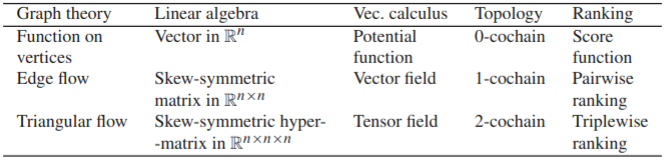
\includegraphics[width=0.8\textwidth]{corresponding.png}
    \caption{数学概念的对应表}
    \label{fig1}
\end{figure}


\section{基于图的统计排序}

\subsection{问题背景与模型构建}

\subsubsection{数据特性与挑战}
现代排名数据（如电商评分、网页链接）具有以下特征：
\begin{itemize}
    \item \textbf{基数评分为主}：区别于传统序数排序，如 Netflix 的 1-5 星评分；
    \item \textbf{高度不完整性}：数据缺失普遍（如 Netflix 数据缺失率达 99\%）；
    \item \textbf{图结构隐含}：对象间关系可建模为图，如用户-商品交互图。
\end{itemize}

\subsubsection{图模型定义}
设：
\begin{itemize}
    \item 顶点集 $V$：待排名对象，$V = \{1, 2, \dots, n\}$；
    \item 选民集 $\Lambda$：评分主体，$\Lambda = \{1, 2, \dots, m\}$；
    \item Pairwise 排名矩阵：对选民 $\alpha$，定义反对称矩阵 $Y^{\alpha} \in \mathbb{R}^{n \times n}$，其中 $Y_{ij}^{\alpha} = -Y_{ji}^{\alpha}$，量化 $i$ 对 $j$ 的偏好强度（如评分差、比率或二元偏好）；
    \item 权重函数：$w_{ij}^{\alpha} = 1$ 表示选民 $\alpha$ 对 $\{i, j\}$ 有有效比较，否则为 0。
\end{itemize}

\subsection{核心模型与优化问题}

\subsubsection{梯度流模型类 $\mathcal{M}_G$}
定义全局一致的 pairwise 排名为梯度流：
$$
X_{ij} = s_j - s_i, \quad \exists s: V \to \mathbb{R}
$$
其中 $s$ 为评分函数，$X \in \mathcal{M}_G$ 确保全局无循环矛盾（如 $i \succ j \succ k \succ i$ 不成立）。

\begin{figure}[H]
    \centering
    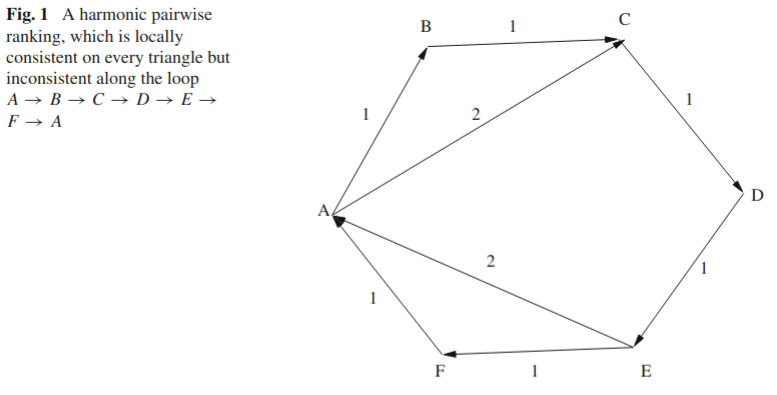
\includegraphics[width=0.8\textwidth]{fig1.png}
    \label{fig2}
\end{figure}

\subsubsection{加权最小二乘损失函数}
目标是将观测边流 $\bar{Y}$ 投影到梯度流空间，最小化加权平方损失：
$$
\min_{s \in \mathbb{R}^n} \sum_{\alpha,i,j} w_{ij}^{\alpha} \left( X_{ij} - Y_{ij}^{\alpha} \right)^2 
= \min_{s \in \mathbb{R}^n} \sum_{\{i,j\} \in E} w_{ij} \left( (s_j - s_i) - \bar{Y}_{ij} \right)^2 
$$
其中：
\begin{itemize}
    \item $w_{ij} = \sum_{\alpha} w_{ij}^{\alpha}$ 为边权重总和；
    \item $\bar{Y}_{ij} = \frac{\sum_{\alpha} w_{ij}^{\alpha} Y_{ij}^{\alpha}}{w_{ij}}$ 为平均偏好强度。
\end{itemize}

\subsection{关键算子与理论工具}

\subsubsection{组合梯度算子（Combinatorial Gradient）}
定义梯度算子 $\text{grad}: \mathbb{R}^n \to \mathbb{R}^{n \times n}$：
$$
(\text{grad } s)(i,j) = s_j - s_i 
$$
性质：梯度流 $\text{grad } s$ 对应全局一致排名，满足 $\text{curl} \circ \text{grad} = 0$（无局部循环矛盾）。

\subsubsection{组合旋度算子（Combinatorial Curl）}
对三角形 $\{i,j,k\} \in T(E)$（3-团），定义旋度算子 $\text{curl}: \mathbb{R}^{n \times n} \to \mathbb{R}^{n \times n \times n}$：
$$
(\text{curl } X)(i,j,k) = X_{ij} + X_{jk} + X_{ki} 
$$
物理意义：量化三角循环矛盾，若 $|\text{curl } X| = 3$，则存在严格循环偏好 $i \succ j \succ k \succ i$。

\subsubsection{霍奇分解定理（Hodge Decomposition）}
任意边流 $X$ 可正交分解为：
$$
X = \text{grad } s + \text{curl}^* \Phi + X_{\text{harmonic}} 
$$
其中：
\begin{itemize}
    \item 梯度流（全局一致）：$\text{grad } s \in \text{im}(\text{grad})$；
    \item 旋度流（局部循环）：$\text{curl}^* \Phi \in \text{im}(\text{curl}^*)$，对应三角矛盾；
    \item 调和流（全局循环）：$X_{\text{harmonic}} \in \ker(\Delta_1)$，对应非三角长程循环；
\end{itemize}
其中$\Delta_1 = \text{curl}^* \circ \text{curl} + \text{grad} \circ \text{div}$ 为 1-维组合拉普拉斯算子；
 $\ker(\Delta_1)$ 的维度等于图的第一贝蒂数 $\beta_1$（拓扑洞数量）。

\subsection{算法求解与性质}

\subsubsection{最小二乘解推导}
对优化问题 (1)，引入图拉普拉斯算子 $\Delta_0 = \text{div} \circ \text{grad}$，其矩阵形式为：
$$
(\Delta_0)_{ij} = 
\begin{cases} 
\sum_k w_{ik}, & i = j \\
-w_{ij}, & i \neq j, \{i,j\} \in E \\
0, & \text{otherwise}
\end{cases}
$$
正规方程为：
$$
\Delta_0 s = -\text{div } \bar{Y} 
$$
其中散度 $\text{div } \bar{Y} = \sum_j w_{ij} \bar{Y}_{ij}$。通过 Moore-Penrose 逆求得最小范数解：
$$
s^* = -\Delta_0^{\dagger} \text{div } \bar{Y}
$$

\subsubsection{不一致性量化}
总残差：
$$
R^* = \bar{Y} - \text{grad } s^* \in \ker(\text{div}) 
$$
满足 $ div\ R^*  = 0 $，表征全局循环矛盾。残差分解：
$$
R^* = \text{proj}_{\text{im}(\text{curl}^)} \bar{Y} + \text{proj}_{\ker(\Delta_1)} \bar{Y}
$$
\begin{itemize}
    \item 局部矛盾：$\text{proj}_{\text{im}(\text{curl}^*)} \bar{Y}$，由三角循环引起；
    \item 全局矛盾：$\text{proj}_{\ker(\Delta_1)} \bar{Y}$，由长程循环引起。
\end{itemize}
循环比率：
$$
C_p = \frac{||R^*||_{2,w}^2}{||\bar{Y}||_{2,w}^2} \times 100\%
$$
衡量不一致性占比，$C_p$ 越小则全局排名越可靠。

\subsection{平均 pairwise 排名}
\paragraph{核心问题}:
原始排名数据常存在高度缺失（如 Netflix 数据缺失率达 99\%），需通过聚合选民偏好生成更完整的 pairwise 排名矩阵。本节介绍四种数据预处理方法，将基数评分或序数排序转化为 pairwise 边流，为后续霍奇分解提供输入。

\paragraph{四种平均 pairwise 排名方法}:
\begin{enumerate}
    \item 算术平均差 \\ 
        \(\alpha\) 的评分差 \(Y_{ij}^{\alpha} = a_{\alpha j} - a_{\alpha i}\)，计算有效比较的算术平均：\(\overline{Y}_{ij} = \frac{\sum_{\alpha} (a_{\alpha j} - a_{\alpha i})}{\#\{\alpha \mid a_{\alpha i}, a_{\alpha j} \text{ exist}\}}\)具有平移不变性，适用于评分绝对差异重要的场景。
    \item 几何平均比 \\
        对评分比 \(Y_{ij}^{\alpha} = \frac{a_{\alpha j}}{a_{\alpha i}}\)，取对数后计算几何平均：\(\overline{Y}_{ij} = \frac{\sum_{\alpha} (\log a_{\alpha j} - \log a_{\alpha i})}{\#\{\alpha \mid a_{\alpha i}, a_{\alpha j} \text{ exist}\}}\)具有尺度不变性，适用于相对比率更重要的场景（如金融汇率）。
    \item 二元比较 \\
    将评分转化为二元偏好 \(Y_{ij}^{\alpha} = \text{sign}(a_{\alpha j} - a_{\alpha i})\)，计算偏好概率差：\(\overline{Y}_{ij} = \text{Pr}\{\alpha \mid a_{\alpha j} > a_{\alpha i}\} - \text{Pr}\{\alpha \mid a_{\alpha j} < a_{\alpha i}\}\)仅保留序数信息，适用于二元决策场景。
    \item 对数优势比 \\
    对二元偏好的概率取对数：\(\overline{Y}_{ij} = \log \frac{\text{Pr}\{\alpha \mid a_{\alpha j} \geq a_{\alpha i}\}}{\text{Pr}\{\alpha \mid a_{\alpha j} \leq a_{\alpha i}\}}\)增强概率差异的对比度，适用于需放大微弱偏好的场景。
\end{enumerate}
\paragraph{方法意义}:\\
\indent \textbf{兼容性：}适用于基数数据（如评分）和序数数据（如偏好排序），通过不同聚合方式保留数据特性。\\
\indent \textbf{降维与补全：}将高维稀疏评分矩阵转化为低维密集的 pairwise 图，缓解数据缺失问题（如 Netflix 数据缺失率从 99\% 降至 0.22\%）。\\
\indent \textbf{预处理灵活性：}可结合领域知识选择权重 \(w_{ij}^{\alpha}\)（如可信度或比较次数），提升后续排名的鲁棒性。
\subsection{应用案例与实验分析}

\subsubsection{Netflix 电影排名}
\paragraph{数据预处理}：
25 部电影 74 个月评分，转化为三种 pairwise 指标：
\begin{enumerate}
    \item 算术平均差：$\bar{Y}_{ij} = \frac{\sum_{\alpha} (a_{\alpha j} - a_{\alpha i})}{n_{\alpha}}$
    \item 几何平均比（对数）：$\bar{Y}_{ij} = \frac{\sum_{\alpha} (\log a_{\alpha j} - \log a_{\alpha i})}{n_{\alpha}}$
    \item 二元比较：$\bar{Y}_{ij} = \text{Pr}(\alpha \text{ prefers } j \text{ over } i) - \text{Pr}(\alpha \text{ prefers } i \text{ over } j)$
\end{enumerate}

\paragraph{结果对比}：
霍奇排名（二元比较）的循环比率 $C_p = 0.30\%$，显著低于简单平均法。排名与独立影评网站 MRQE 的 Kendall $\tau$ 距离最小，验证可靠性。

\subsubsection{货币兑换市场验证}
\paragraph{模型设定}：
7 种货币汇率构成完全图，对数变换后 $X_{ij} = \log a_{ij}$，要求无三角套利（$\text{curl } X = 0$）。

\paragraph{结论}：
当 $\text{curl } X = 0$ 时，存在全局价格函数 $\pi_i = e^{-s_i}$，满足 $a_{ij} = \pi_j / \pi_i$。完全图中 $\beta_1 = 0$，调和流为零，局部一致蕴含全局一致。

\subsection{理论价值与创新}

\subsubsection{方法论突破}
\begin{itemize}
    \item \textbf{拓扑视角}：通过组合霍奇理论，将数据矛盾与图的拓扑特征（如贝蒂数）关联，首次建立 “循环矛盾→拓扑洞” 的数学对应；
    \item \textbf{计算效率}：线性最小二乘求解（$O(n^3)$）替代 NP-hard 的 Kemeny 优化，适用于大规模数据。
\end{itemize}

\subsubsection{公式总结}
\begin{center}
\begin{tabular}{ccc}
符号 & 公式 & 含义 \\ \hline
梯度流 & $X_{ij} = s_j - s_i$ & 全局一致排名 \\
旋度 & $(\text{curl } X)_{ijk} = X_{ij} + X_{jk} + X_{ki}$ & 三角循环检测 \\
霍奇分解 & $X = \text{grad } s + \text{curl}^* \Phi + X_{\text{harmonic}}$ & 正交分解边流 \\
正规方程 & $\Delta_0 s = -\text{div } \bar{Y}$ & 最小二乘解
\end{tabular}
\end{center}


\section{矩阵视角下的霍奇分解理论}
\subsection{斜对称矩阵空间}
\indent \textbf{定义：}矩阵 $X \in \mathbb{R}^{n \times n}$ 是斜对称的，若 $X_{ij} = -X_{ji} \ (\forall i,j)$。\\
\indent \textbf{空间分解:}全体斜对称矩阵构成空间 $\mathcal{A}$，对称矩阵构成空间 $\mathcal{S}$:$\mathcal{A} := \{ X \mid X^\top = -X \}, \quad \mathcal{S} := \{ X \mid X^\top = X \}.$\\
\indent \textbf{一般矩阵分解：}任意方阵 $A$ 可唯一分解为对称与斜对称部分：$A = \frac{1}{2}(A + A^\top) + \frac{1}{2}(A - A^\top).$

\subsection{梯度矩阵(Gradient Matrices)}
\indent \textbf{构造:}给定向量 $s = [s_1, \ldots, s_n]^\top$，定义斜对称矩阵：$X_{ij} := s_i - s_j.$\\
\indent \textbf{性质：}   
\begin{itemize}
    \item 非零时秩恒为 2（因 $X = se^\top - es^\top$，其中 $e = [1, \ldots, 1]^\top$）。
    \item 是秩最小的非零斜对称矩阵（斜对称矩阵秩必为偶数）。
\end{itemize}
\indent \textbf{梯度矩阵空间：}$\mathcal{M}_G := \{ X \in \mathcal{A} \mid X_{ij} = s_i - s_j \text{ for some } s \in \mathbb{R}^n \}.$

\subsection{T-一致矩阵（T-Consistent Matrices）}
\indent \textbf{定义：}对三角集 $T \subseteq \binom{V}{3}$（所有三元组），定义：
\begin{equation}
\mathcal{M}_T := \{ X \in \mathcal{A} \mid X_{ij} + X_{jk} + X_{ki} = 0, \forall \{i,j,k\} \in T \}.
\end{equation}
\indent \textbf{关键关系：} \begin{itemize}
    \item 梯度矩阵必满足任意 $T$ 的一致性：$\mathcal{M}_G \subseteq \mathcal{M}_T$。
    \item 当 $T = \binom{V}{3}$（全体三元组）时，一致性条件等价于梯度矩阵：
    \begin{equation}
    \mathcal{M}_G = \mathcal{M}_{\binom{V}{3}}.
    \end{equation}
\end{itemize}

\subsection{子空间包含关系}
\begin{equation}
    \mathcal{M}_G \subseteq \mathcal{M}_T \subseteq \mathcal{A}.
\end{equation}
    
    \begin{itemize}
        \item $\mathcal{M}_G$ 和 $\mathcal{M}_T$ 均为 $\mathbb{R}^{n \times n}$ 的子空间。
        \item 一般包含关系严格，故可定义正交补空间。
    \end{itemize}

\subsection{正交分解与调和矩阵}
在标准内积 $\langle X, Y \rangle = \text{tr}(X^\top Y)$ 下：

\begin{enumerate}
    \item 空间分解：
    $$
    \mathcal{A} = \mathcal{M}_G \oplus \mathcal{M}_G^\perp, \quad \mathcal{A} = \mathcal{M}_T \oplus \mathcal{M}_T^\perp.
    $$
    
    \item $\mathcal{M}_T$ 的分解：
    $$
    \mathcal{M}_T = \mathcal{M}_G \oplus \mathcal{M}_H, \quad \text{其中} \quad \mathcal{M}_H := \mathcal{M}_T \cap \mathcal{M}_G^\perp.
    $$
    \begin{itemize}
        \item $\mathcal{M}_H$ 称为调和矩阵空间，是离散 Laplace 方程（或 Helmholtz 方程）的解的类比。
        \item 调和矩阵的物理意义：无旋（curl-free）且无散（divergence-free）。
    \end{itemize}
\end{enumerate}

\subsection{霍奇分解定理（矩阵形式）}
斜对称矩阵空间的正交直和分解：

\begin{equation}
\boxed{\mathcal{A} = \mathcal{M}_G \oplus \mathcal{M}_H \oplus \mathcal{M}_T^\perp}.
\tag{18}
\end{equation}

对应物理意义：
\begin{itemize}
    \item $\mathcal{M}_G$: 梯度流（无旋场）。
    \item $\mathcal{M}_H$: 调和流（harmonic 场）。
    \item $\mathcal{M}_T^\perp$: 旋度流（curl 场）。
\end{itemize}

\section{组合霍奇理论}
\subsection{单纯复形（Simplicial Complex）}

    \indent \textbf{背景}：为描述三角不一致性（旋度），需将成对比较图 \(G = (V, E)\) 扩展为二维单纯复形：
    \[
    K_G^3 = (V, E, T(E)), \quad T(E) := \left\{ \{i,j,k\} \in \binom{V}{3} \mid \{i,j\},\{j,k\},\{k,i\} \in E \right\}
    \]
    \begin{itemize}
        \item \(T(E)\) 是图 \(G\) 中所有3-团（三角形）的集合。
    \end{itemize}
    
    \indent \textbf{一般定义}：单纯复形 \((V, \Sigma)\) 由顶点集 \(V\) 和\textbf{对子集封闭}的单纯形集合 \(\Sigma\) 构成：
    \begin{itemize}
        \item \(k\)-单纯形：\(\Sigma_k \subseteq \binom{V}{k+1}\)（如0-单形为顶点，1-单形为边，2-单形为三角形）
        \item \textbf{团复形}：图 \(G\) 的 \(k\)-团复形 \(K_G^k\) 由所有 \(j\)-团（\(j=1,\dots,k\)）构成。
    \end{itemize}


\subsection{上同调群（Cochains）与算子}
\indent \textbf{上链空间}（定义在单纯复形 \(K\) 上）：
    \begin{itemize}
        \item \(C^0\)：顶点函数（分数函数）\(s: V \to \mathbb{R}\)
        \item \(C^1\)：边流（成对排序）\(X: E \to \mathbb{R}\)，满足 \(X_{ij} = -X_{ji}\)
        \item \(C^2\)：三角流 \(\Phi: T \to \mathbb{R}\)，满足完全反对称性
    \end{itemize}
    
    \indent\textbf{内积}（统计排序背景）：
    \[
    \langle X, Y \rangle_w = \sum_{\{i,j\} \in E} w_{ij} X_{ij} Y_{ij}, \quad w_{ij} > 0 \text{ 当 } \{i,j\} \in E
    \]
    
    \indent \textbf{上边缘算子}（关键映射）：
    \begin{itemize}
        \item \textbf{梯度}：\(\delta_0 = \text{grad}\)  
        \[
        (\text{grad } s)(i,j) = s_j - s_i
        \]
        \item \textbf{旋度}：\(\delta_1 = \text{curl}\)  
        \[
        (\text{curl } X)(i,j,k) = X_{ij} + X_{jk} + X_{ki}
        \]
        \item \textbf{散度}（伴随算子）：\(\text{div} = -\delta_0^*\)  
        \[
        (\text{div } X)(i) = \sum_{j: \{i,j\} \in E} w_{ij} X_{ij}
        \]
    \end{itemize}

\subsection{组合拉普拉斯算子（Combinatorial Laplacian）}
\indent \textbf{定义}：
    \[
    \Delta_k = \delta_k^* \circ \delta_k + \delta_{k-1} \circ \delta_{k-1}^*
    \]
    \begin{itemize}
        \item \textbf{图拉普拉斯算子}（\(k=0\)）：\(\Delta_0 = -\text{div} \circ \text{grad}\)
        \item \textbf{图亥姆霍兹算子}（\(k=1\)）：\(\Delta_1 = \text{curl}^* \circ \text{curl} - \text{grad} \circ \text{div}\)
    \end{itemize}
    
    \indent \textbf{性质}：
    \begin{itemize}
        \item 半正定算子：\(\Delta_k \succeq 0\)
        \item \(\ker(\Delta_k)\) 的维数等于复形 \(K\) 的第 \(k\) 维贝蒂数（拓扑不变量）
    \end{itemize}

\subsection{霍奇分解定理（Hodge Decomposition）}
\indent \textbf{一般形式}（对任意 \(k\)）：
    \[
    C^k = \operatorname{im}(\delta_{k-1}) \oplus \ker(\Delta_k) \oplus \operatorname{im}(\delta_k^*)
    \]
    \[
    \ker(\Delta_k) = \ker(\delta_k) \cap \ker(\delta_{k-1}^*)
    \]
    
    \indent \textbf{亥姆霍兹分解}（\(k=1\)，成对排序场景）：
    \[
    \boxed{
    C^1 = \underbrace{\operatorname{im}(\text{grad})}_{\text{梯度流}} \oplus \underbrace{\ker(\Delta_1)}_{\text{调和流}} \oplus \underbrace{\operatorname{im}(\text{curl}^*)}_{\text{旋度流}}
    }
    \]
    \[
    \ker(\Delta_1) = \ker(\text{curl}) \cap \ker(\text{div})
    \]
    \begin{figure}[h]
        \centering
        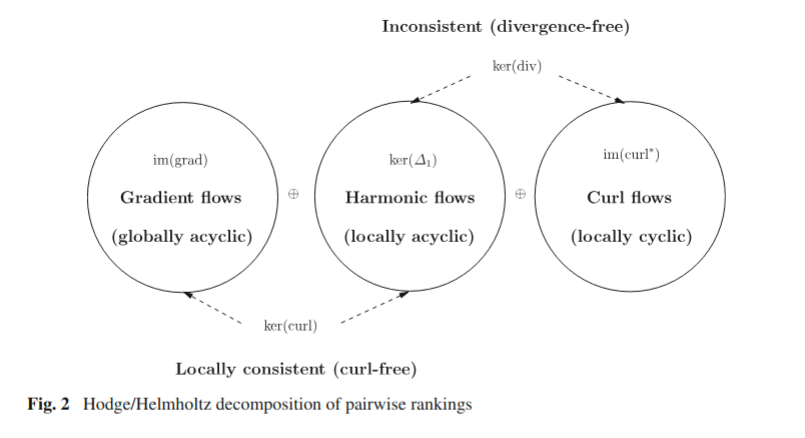
\includegraphics[width=0.8\textwidth]{4.3th2.png}
        \caption{亥姆霍兹分解的图示}
    \end{figure}

\subsection{子空间的排序解释（HodgeRank）}
\begin{center}
    \begin{tabular}{|l|l|l|}
        \hline
        \textbf{子空间} & \textbf{数学条件} & \textbf{排序意义} \\
        \hline
        梯度流 \(\operatorname{im}(\text{grad})\) & \(X = \text{grad } s\) & 全局一致：存在分数 \(s\) 诱导全局排序（无旋） \\
        \hline
        调和流 \(\ker(\Delta_1)\) & \(\begin{cases} \text{curl } X = 0 \\ \text{div } X = 0 \end{cases}\) & 局部一致但全局不一致：无三角形环，但存在长度 >3 的环 \\
        \hline
        旋度流 \(\operatorname{im}(\text{curl}^*)\) & \(X \perp \ker(\text{div})\) & 局部不一致：存在三角形环（如 \(i>j>k>i\)） \\
        \hline
    \end{tabular}
\end{center}

\subsection{几何与物理类比}
\begin{itemize}
    \item \textbf{闭链性}（Closedness）：\(\delta_{k+1} \circ \delta_k = 0\)  $→$ \(\text{curl} \circ \text{grad} = 0\)（全局一致蕴含局部一致）
    \item \textbf{调和流}：离散亥姆霍兹方程的解 \(\Delta_1 X = 0\)，类比连续场的无旋无散条件。
    \item \textbf{拓扑障碍}：\(\dim \ker(\Delta_1)\) 反映图中不可缩环的数量（调和流的自由度）。
\end{itemize}


\section{HodgeRank分析}
\subsection{全局排序与不一致残差的结构分解}

\subsubsection{优化问题的数学本质}

\begin{itemize}
    \item 最小二乘问题:
    $$
    \min_{s \in C^0} \| \text{grad } s - \bar{Y} \|_{2,w}^2 \iff \delta_0^* \delta_0 s = \delta_0^* \bar{Y}
    $$
    \begin{itemize}
        \item 法方程: $\Delta_0 s = -\text{div} \bar{Y}$ (由 $\Delta_0 = \delta_0^* \delta_0$, $\text{div} = -\delta_0^*$)
        \item 唯一解: $s^* = -\Delta_0^\dagger \text{div} \bar{Y}$ (Moore-Penrose逆保证最小范数)
    \end{itemize}
    
    \item 算子显式形式:
    \begin{table}[h]
        \centering
        \begin{tabular}{m{4cm} m{6cm} m{6cm}}
            \textbf{算子} & \textbf{定义} & \textbf{矩阵表示} \\
            \hline
            散度 div & $(\text{div} \bar{Y})(i) = \sum_j w_{ij} \bar{Y}_{ij}$ & 加权邻接矩阵的行和 \\
            \hline
            图拉普拉斯 $\Delta_0$ & 
            $[\Delta_0]_{ij} = 
            \begin{cases} 
                \sum_k w_{ik} & i = j \\
                -w_{ij} & \{i,j\} \in E \\
                0 & \text{else}
            \end{cases}$ & 对称半正定矩阵 \\
        \end{tabular}
    \end{table}
\end{itemize}
\subsubsection{残差的正交分解与物理意义}

\begin{itemize}
    \item 无散性: $R^* = \bar{Y} - \text{grad } s^*$ 满足 $\text{div } R^* = 0$
    
    \item Helmholtz分解:
    $$
    R^* = \underbrace{\text{curl}^* \Phi^*}_{\text{局部循环}} + \underbrace{(I - \Delta_1^\dagger \Delta_1) \bar{Y}}_{\text{调和分量}}
    $$
    \begin{itemize}
        \item 投影算子:
        \begin{itemize}
            \item (局部不一致性)
            \item $\text{proj}_{\ker(\Delta_1)} = I - \Delta_1^\dagger \Delta_1$ (全局拓扑不一致性)
        \end{itemize}
        
        \item 正交性: $\text{im}(\text{grad}) \perp \text{im}(\text{curl}^*) \oplus \ker(\Delta_1)$
    \end{itemize}
\end{itemize}
\subsubsection{实际案例：Borda计分的推广}

\begin{itemize}
    \item 完全图特例（无缺失数据）:
    $$
    s_i^* = -\frac{1}{n} \sum_j \bar{Y}_{ij}, \quad \text{即经典Borda计分}
    $$
    
    \item 现实限制: 现代排名数据通常高度稀疏（如Netflix >99\%缺失值），HodgeRank通过加权图拉普拉斯 $\Delta_0$ 泛化至非完全图。
\end{itemize}

\subsubsection{调和分量的稀疏化处理}

\begin{itemize}
    \item NP难问题: $\min_{\Phi} \| \text{curl}^* \Phi - R^* \|_0$ （寻找最简冲突边集）
    
    \item 凸松弛方案:
    $$
    \min_{\Phi \in C^2} \sum_{\{i,j\}} |(\text{curl}^* \Phi)_{ij} - R_{ij}^*| \quad (l_1-\text{范数替代})
    $$
    \begin{itemize}
        \item 目标: 识别最小“冲突三角”集合，移除后使图全局一致
        \item 类比: 最小反馈弧集（见第6.2节）
    \end{itemize}
\end{itemize}

\subsubsection{计算复杂度与优化}

\begin{table}[h]
    \centering
    \begin{tabular}{m{4cm} m{4cm} m{3cm} m{6cm}}
        \textbf{组件} & \textbf{计算任务} & \textbf{复杂度} & \textbf{优化策略} \\
        \hline
        全局排序 $s^*$ & $n \times n$ 最小二乘 & $O(n^3)$ & 共轭梯度法 \\
        \hline
        局部循环分量 & 计算 $\text{curl}$ & $O(|T|)$ & 三角关系稀疏存 \\
        \hline
        调和分量 $\text{proj}_{\ker(\Delta_1)}$ & $(T \times T)$ 最小二乘 & 最坏$O(n^9)$ & LSQR / MINRES-QLP\\
    \end{tabular}
\end{table}

\textbf{注：} 实际中 $|T| \ll \binom{n}{3}$（如Netflix的边缺失率仅0.22\%），可利用稀疏性加速。

\subsection{局部一致性与全局一致性的等价条件}

\textbf{定理4：拓扑决定的一致性等价}

\begin{itemize}
    \item 核心结论: 若3-团复形 $K_G^3$ 的一维贝蒂数 $\beta_1(K_G^3) = 0$（无1维环），则:
    $$
    \text{curl}(X) = 0 \quad (\text{局部三角一致}) \implies X = \text{grad } s \quad (\text{全局一致})
    $$
    
    \item 证明关键:
    \begin{itemize}
        \item 由Helmholtz分解: $\ker(\Delta_1) \oplus \text{im}(\text{curl}^*) = \text{im}(\text{grad})^\perp$
        \item $\beta_1 = \dim \ker(\Delta_1) = 0$ 时, $\text{im}(\text{curl}^*) = \text{im}(\text{grad})^\perp \rightarrow$ 无调和空间
    \end{itemize}
\end{itemize}
\textbf{随机图拓扑分析（Kahle定理）}

\begin{itemize}
    \item Erdős-Rényi图 $G(n,p)$:
    $$
    \beta_1(K_G) = 0 \quad \text{几乎必然成立}, \quad \text{除非} \quad \frac{1}{n^2} \ll p \ll \frac{1}{n}
    $$
    \begin{itemize}
        \item 相变解释:
        \begin{itemize}
            \item $p \ll 1/n$: 边过稀，无三角结构
            \item $p \gg 1/n$: 边稠密，三角覆盖充分
            \item $1/n^2 \ll p \ll 1/n$: 存在环状拓扑 ($\beta_1 > 0$)
        \end{itemize}
    \end{itemize}
    
    \item Netflix案例验证:
    \begin{itemize}
        \item 顶点数 $n \approx 480,000$ （电影数）
        \item 边密度 $p \approx 1 - 0.0022 = 0.9978$
        \item 条件判断: $p \gg 1/n \approx 2 \times 10^{-6} \rightarrow$ 几乎必然 $\beta_1 = 0$
    \end{itemize}
\end{itemize}


\section{社会选择理论的关联}
\subsection{Kemeny优化与Borda计分的数学本质}

\subsubsection{经典方法回顾}

\begin{table}[h]
    \centering
    \begin{tabular}{m{1.5cm} m{4cm} m{2.5cm} m{2cm} m{3cm}}
        \textbf{方法} & \textbf{数学形式} & \textbf{假设条件} & \textbf{复杂度} & \textbf{局限} \\
        \hline
        Kemeny优化 & $\min_{\sigma} \sum_{i=1}^{m} d_K(\sigma, \tau_i); $
            $d_K = \frac{1}{4} \sum_{i,j} \| Y_{ij}^{\sigma} - Y_{ij}^{\tau} \|$
        & 完全图、平衡权重、二元数据 & NPH & 忽略基数信息，仅用序数关系 \\
        \hline
        Borda计分 & $s_B(i) = -\sum_{\alpha,k} Y_{ik}^{\alpha}$ & 完全图、平衡权重、二元数据 & $O(n^2)$ & 不满足Condorcet准则与淘汰一致性 \\
    \end{tabular}
\end{table}

\textbf{传统假设的缺陷:}

\begin{itemize}
    \item Netflix案例: 99\%数据缺失 $\rightarrow$ 非完全（用户未评全电影）、非平衡（热门电影权重高）、基数数据（1-5星）
    \item 后果: 经典方法直接应用会导致信息损失（如5星vs\ 1星 $\equiv$ 3星vs\ 2星）或不可计算。
\end{itemize}

\subsubsection{HodgeRank的推广与退化}

\begin{itemize}
    \item 广义Borda计分（适应现代数据）:
    $$
    s^*(i) = -\Delta_0^\dagger \text{div} \bar{Y} \quad (\text{加权图拉普拉斯逆})
    $$
    \begin{itemize}
        \item 关键改进:
        \begin{itemize}
            \item 处理非完全图（通过 $\Delta_0$ 的稀疏结构）
            \item 适应非平衡权重 ($w_{ij}$ 反映数据置信度)
            \item 保留基数信息（直接使用评分差值 $Y_{ij}^\alpha$）
        \end{itemize}
    \end{itemize}
    
    \item 经典Borda的退化:
    当数据完全、平衡且二元时 ($w_{ij} = c$, $Y_{ij}^\alpha \in \{\pm1\}$):
    $$
    s^*(i) \propto -\sum_{j,\alpha} Y_{ij}^\alpha = s_B(i) \quad (\text{与Borda等价})
    $$
\end{itemize}

\subsubsection{Kemeny优化的Hodge表述}

\begin{itemize}
    \item 离散模型类: $\mathcal{M}_K = \{X \mid X_{ij} = \text{sign}(s_j - s_i)\}$
    
    \item 最小二乘形式:
    $$
    \min_{X \in \mathcal{M}_K} \sum_{\alpha,i,j} w_{ij}^\alpha (X_{ij} - Y_{ij}^\alpha)^2
    $$
    $\rightarrow$ 计数成对排序冲突数（与Kemeny目标等价）
\end{itemize}

\subsection{等价性定理与几何解释}

\textbf{定理6：四类优化问题的等价性（二元数据 $Y_{ij}^\alpha \in \{\pm1\}$）}

\begin{table}[h]
    \centering
    \begin{tabular}{m{3cm} m{7cm} m{5cm}}
        \textbf{问题形式} & \textbf{数学描述} & \textbf{实际意义} \\
        \hline
        (i) 最小二乘 & $\min_{X \in \mathcal{M}_K} \sum w_{ij}^\alpha (X_{ij} - Y_{ij}^\alpha)^2$ & Kemeny冲突数最小化 \\
        \hline
        (ii) 线性规划 & $\max_{X \in \mathcal{K}_1} \sum w_{ij} X_{ij} \bar{Y}_{ij}$ & 凸包上的效用最大化 \\
        \hline
        (iii) 加权$L_1$投影 & $\min_{X \in \mathcal{K}_2} \sum w_{ij} \|X_{ij} - \bar{Y}_{ij}\|$ & 到可传递区域的最小曼哈顿距离 \\
        \hline
        (iv) 最小反馈弧集 & 删除边集使图无环，且边权重和最小 & 消除最小冲突比较边 \\
    \end{tabular}
\end{table}

\subsection*{证明思路:}

\begin{enumerate}
    \item (i)$\Leftrightarrow$(ii): 因 $\mathcal{M}_K$ 离散，线性规划在其凸包 $\mathcal{K}_1$ （置换矩阵凸组合）上求解。
    
    \item (i)$\Leftrightarrow$(iv): 最小二乘目标等价于最大化 $\sum w_{ij} X_{ij} \bar{Y}_{ij} \rightarrow$ 反转边方向使图无环 $\rightarrow$ 最小反馈弧集。
    
    \item (iii)$\Leftrightarrow$(iv): 加权$L_1$投影的解 $X_{ij}^* \in \{0, \pm1\} \rightarrow$ 删除 $X_{ij}^* = 0$ 的边即得反馈弧集。
\end{enumerate}
\begin{figure}[h]
    \centering
    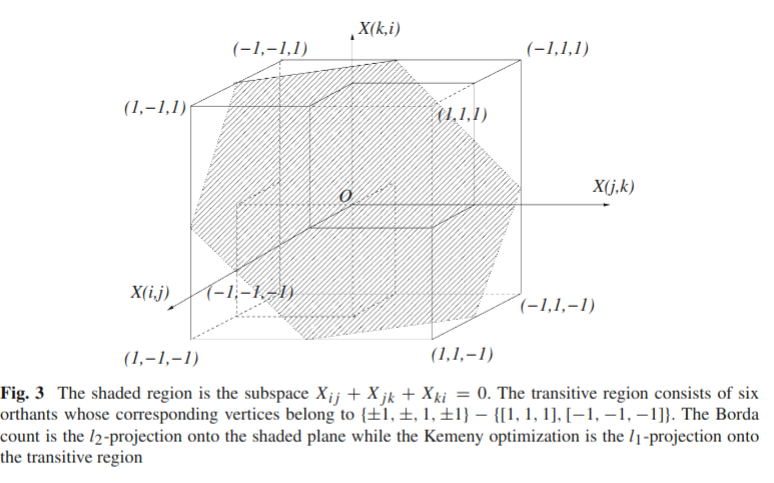
\includegraphics[width=0.8\textwidth]{6.2below.png}
\end{figure}
\begin{tikzpicture}[node distance=2cm, auto]
    % Define nodes
    \node (A) [rectangle, draw] {数据空间 $[-1,1]^3$};
    \node (B) [rectangle, draw, below of=A, left of=A, node distance=4cm] {可传递区域 $K_2$};
    \node (C) [rectangle, draw, below of=A, right of=A, node distance=4cm] {梯度流平面 $M_G$};
    \node (D) [rectangle, draw, below of=B, node distance=3.5cm] {6个象限-顶点 excl $(-1,-1,-1)$ 和 $(1,1,1)$};
    \node (E) [rectangle, draw, below of=C, node distance=3.5cm] {平面 $X_{ij} + X_{jk} + X_{ki} = 0$};
    \node (F) [rectangle, draw, below of=D, node distance=3.5cm] {Kemeny优化 - L1投影到 $K_2$};
    \node (G) [rectangle, draw, below of=E, node distance=3.5cm] {HodgeRank - L2投影到 $M_G$};

    % Draw edges
    \draw[->] (A) -- (B);
    \draw[->] (A) -- (C);
    \draw[->] (B) -- (D);
    \draw[->] (C) -- (E);
    \draw[->] (D) -- (F);
    \draw[->] (E) -- (G);
\end{tikzpicture}\\
\textbf{需要注意的是:}
\begin{itemize}
    \item $K_2$ 包含 $n!$ 个锥（每置换对应一锥）
    \item $M_G$ 是 $K_2$ 的仿射包（三点时即平面 $X_{ij} + X_{jk} + X_{ki} = 0$）
    \item Kemeny优化是 $L_1$ 投影到离散区域，HodgeRank是 $L_2$ 投影到连续子空间
\end{itemize}

\subsection{社会选择性质对比 (Saari-Merlin定理)}

\textbf{定理7：Kemeny与Borda的互约束关系}

对任意投票数据:
\begin{itemize}
    \item Kemeny胜者（最优项）在Borda计分中严格高于Kemeny败者（最劣项）
    \item Borda胜者在Kemeny排序中严格高于Borda败者（但二者中间项排序可能任意不同）
\end{itemize}

\subsubsection*{准则满足性对比}

\begin{table}[h]
    \centering
    \begin{tabular}{m{4cm} m{2cm} m{2cm} m{2cm}}
        \textbf{性质} & \textbf{Kemeny优化} & \textbf{Borda计分} & \textbf{HodgeRank} \\
        \hline
        Condorcet准则 & $\checkmark$ & X (仅胜>败) & $\checkmark$ \\
        \hline
        淘汰一致性 & $\checkmark$ & X & $\checkmark$ \\
        \hline
        基数信息保留 & X & X & $\checkmark$ \\
        \hline
        计算复杂度 & NP难 & $O(n^2)$ & $O(n^3)$ \\
        \hline
        稀疏数据适应性 & X & X & $\checkmark$ \\
    \end{tabular}
\end{table}

\textbf{注:}
\begin{itemize}
    \item Condorcet胜者: $\forall j \neq i$, $\text{sign}(\sum_\alpha Y_{ij}^\alpha) = 1$ （全胜项）
    \item 淘汰一致性: 从 $V$ 移除部分项后，剩余项的全局排序不变
\end{itemize}

\subsubsection*{实际应用启示}

\begin{enumerate}
    \item Kemeny适用场景:
    \begin{itemize}
        \item 数据量小 ($n \leq 10$)
        \item 需严格满足社会选择公理（如选举系统）
    \end{itemize}
    
    \item HodgeRank优势:
    \begin{itemize}
        \item 大规模稀疏数据（如Netflix: $n \approx 48 \times 10^4$, $O(n^3)$ 可行）
        \item 需保留评分强度信息（星级差异）
        \item 高边密度下调和分量消失 ($\beta_1 = 0$) $\rightarrow$ 局部一致性保证全局可靠
    \end{itemize}
\end{enumerate}

\section{实验研究}
\subsection{实验一：Netflix电影排名}

\subsubsection*{目标}

验证HodgeRank在存在时间漂移偏差的数据中生成全局排名的有效性，并通过旋度（curl）量化不一致性。

\subsubsection*{数据}

\begin{itemize}
    \item 选取Netflix数据集中74个月均被评分的25部电影（最终聚焦6部时间漂移明显的电影，如图4）。
    \item 使用三种配对比较统计量:
    \begin{itemize}
        \item 分数差的算术平均（Hodge-difference）
        \item 分数比的几何平均（Hodge-ratio）
        \item 二元比较（Hodge-binary）
    \end{itemize}
\end{itemize}

\begin{figure}[h]
    \centering
    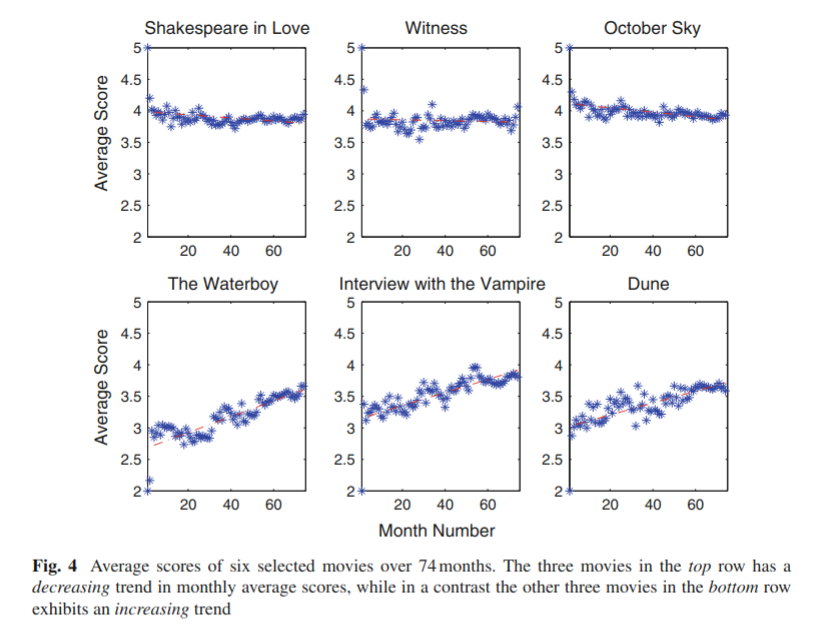
\includegraphics[width=0.8\textwidth]{7.1.png}
    \caption{Netflix数据集中6部电影的评分时间序列}
    \label{fig:netflix_movies}
\end{figure}

\begin{figure}[h]
    \centering
    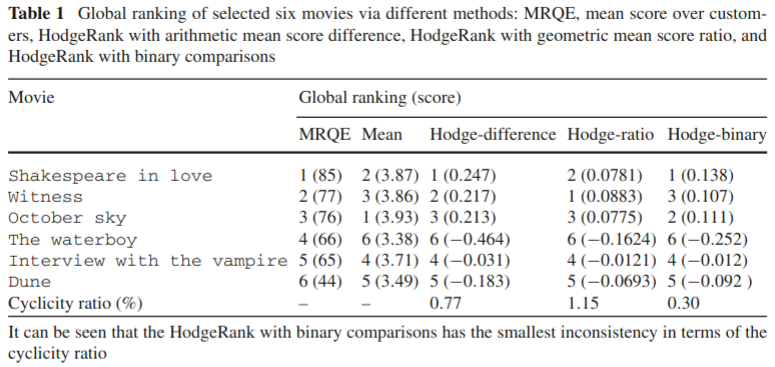
\includegraphics[width=0.8\textwidth]{table1.png}
    \caption{HodgeRank在Netflix数据集上的排名结果}
    \label{fig:hodge_rank_results}
\end{figure}
\subsubsection*{结果}

\indent \textbf{1. 时间漂移鲁棒性}
\begin{itemize}
    \item 简单平均分排名（Mean）与专业影评网站MRQE差异大（如《The Waterboy》排名倒数第1 vs. 第4）。
    \item HodgeRank结果更接近MRQE参考排名（表1）。
\end{itemize}

\indent \textbf{2. 不一致性检测}
\begin{itemize}
    \item 循环比率（Cyclicity Ratio）: 量化全局不一致性，二元比较法最低（0.30\%）。
    \item 相对旋度（Relative Curl）: 定位局部不一致性。
    \begin{itemize}
        \item 边 $\{\text{Witness}, \text{October Sky}\}$ 的旋度异常高（>3.6），导致两者排名不稳定（表1中排名波动）。
    \end{itemize}
\end{itemize}



\subsection{实验二：货币汇率市场}

\subsubsection*{目标}

验证汇率市场的无套利一致性（即配对排名是否可全局整合）。

\subsubsection*{数据}

\begin{itemize}
    \item 7种货币（USD/JPY/EUR等）的汇率（表2），构建完全图。
\end{itemize}

\subsubsection*{方法}

\begin{itemize}
    \item 汇率取对数 $\rightarrow$ 转化为边流（edge flow）。
    \item 求解全局排名 $s^*$ $\rightarrow$ 得通用等价函数 $\exp(-s^*)$ （表2末行）。
\end{itemize}

\subsubsection*{结论}
\begin{figure}[h]
    \centering
    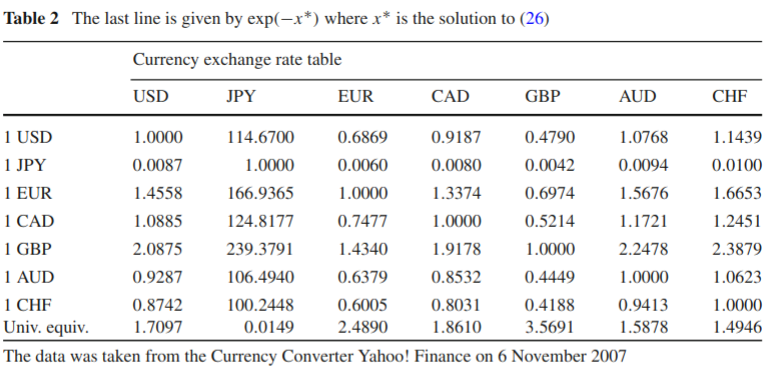
\includegraphics[width=0.8\textwidth]{table2.png}
    \caption{HodgeRank在货币汇率市场的排名结果}
\end{figure}
\begin{itemize}
    \item 对数转换后旋度趋近零（机器精度级别），证明无三角套利机会。
    \item 图结构完全 $\rightarrow$ 局部一致性（无三角套利）蕴含全局一致性（无任意周期套利）。
\end{itemize}

\subsection{实验三：与PageRank/HITS对比}

\subsubsection*{目标}

将HodgeRank应用于网页排名，对比传统方法（PageRank/HITS）。

\subsubsection*{数据}

\begin{itemize}
    \item 英国107所大学的链接结构（2002年） + RAE 2001研究评分。
\end{itemize}

\subsubsection*{方法}

\begin{enumerate}
    \item 定义边流: $Y_{ij} = \log(P_{ij}/P_{ji})$，其中 $P_{ij}$ 为PageRank转移概率。
    \item 可逆马尔可夫链逼近:
    \begin{itemize}
        \item Hodge投影得到 $s^*$ $\rightarrow$ 逼近PageRank的稳态分布 $\pi^*$ ($\pi_i^* \propto e^{s_i^*}$)。
    \end{itemize}
    \item 计算效率:
    \begin{itemize}
        \item HodgeRank只需解最小二乘问题（图拉普拉斯矩阵），计算成本低于PageRank特征值分解。
    \end{itemize}
\end{enumerate}

\subsection*{结果（表3 Kendall $\tau$距离）}
\begin{figure}[h]
    \centering
    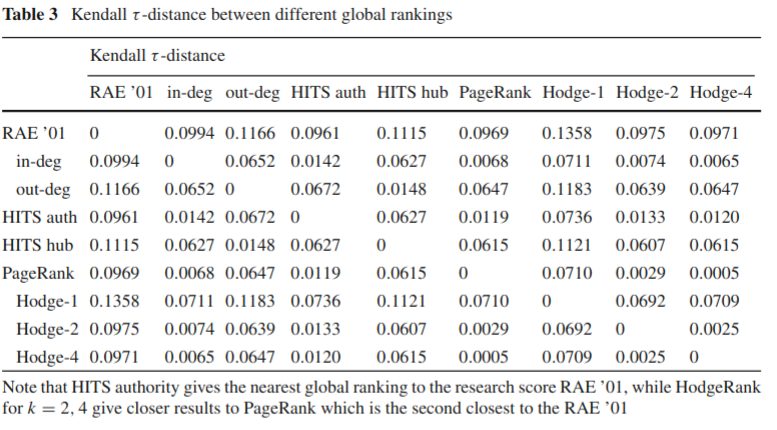
\includegraphics[width=0.8\textwidth]{table3.png}
    \caption{HodgeRank与PageRank/HITS的排名对比}
\end{figure}
\begin{itemize}
    \item 接近RAE研究评分: HITS权威排名最优，PageRank次优。
    \item 逼近PageRank: 高阶HodgeRank（$k=2,4$迭代流）与PageRank距离更小（$\tau \approx 0.0025$）。
    \item 不一致性分析: 旋度可量化PageRank模型的循环性（非可逆性）。
\end{itemize}

\section{总结与展望}
\subsection{核心方法：霍奇理论驱动的排名框架}
\subsubsection{霍奇排名（HodgeRank）的核心思想}
\indent \textbf{建模基础：}将选民对对象的评分转化为图上的边流（edge flow），用反对称矩阵表示两两偏好强度，构建 pairwise 比较图。\\

\indent \textbf{核心分解：}利用组合霍奇理论将边流正交分解为三部分：
\begin{enumerate}
    \item \textbf{梯度流（Gradient Flow）：}对应全局一致排名，通过 \(l_2\) 投影求解最优评分函数 s，即 \(X_{\text{grad}} = \text{grad } s\)，确保无循环矛盾。
    \item \textbf{旋度流（Curl Flow）：}刻画局部三角循环矛盾（如 Condorcet 悖论），对应三角形内的不一致性，通过旋度算子 \(\text{curl}\) 量化。
    \item \textbf{调和流（Harmonic Flow）：}捕捉全局长程循环矛盾，满足局部无旋（\(\text{curl } X = 0\)）但全局发散，与图的拓扑结构（如贝蒂数 \(\beta_1\)）相关。
\end{enumerate}

\subsubsection{与经典方法的联系}
\indent \textbf{对 Borda 计数的推广：}当数据完整、平衡时，霍奇排名的全局分量退化为传统Borda 计数，证明其为序数排名方法在基数数据、缺失场景下的自然扩展。\\
\indent \textbf{计算优势：}避免 Kemeny 优化的 NP 难问题，通过线性最小二乘（\(O(n^3)\) 复杂度）实现高效求解，适用于大规模数据。

\subsection{数据特性与分解的几何意义}
\subsubsection{数据兼容性与矛盾量化}
\indent \textbf{处理复杂数据：}
\begin{enumerate}
    \item \textbf{基数与序数兼容：}通过算术平均差、二元比较等预处理方法，将评分或排序转化为边流，适应不同数据类型。
    \item \textbf{缺失与不平衡处理：}利用图的稀疏性（边权重 \(w_{ij}\)）自然处理缺失值，通过加权内积 \(\langle X, Y \rangle_w = \sum w_{ij}X_{ij}Y_{ij}\) 平衡数据偏差。
\end{enumerate}
\indent \textbf{可靠性 “证书”：}
\begin{enumerate}
    \item \textbf{残差分析：}总残差 \(R^* = \bar{Y} - X_{\text{grad}}\) 的 \(l_2\) 范数衡量全局排名有效性，残差越小，排名可信度越高。
    \item \textbf{矛盾分解：}残差进一步分解为旋度流（局部矛盾）与调和流（全局矛盾），量化不同类型的不一致性。
\end{enumerate}

\subsubsection{图结构与拓扑的作用}
\indent \textbf{组合拉普拉斯算子：}引入图亥姆霍兹算子（Graph Helmholtzian） \(\Delta_1 = \text{curl}^* \circ \text{curl} - \text{grad} \circ \text{div}\)，其核空间（调和流）维度等于图的第一贝蒂数 \(\beta_1\)，刻画图的 “拓扑洞”（如长程循环）。

\indent \textbf{一致性条件：}当图的 3 - 团复形无拓扑洞（\(\beta_1 = 0\)）时，局部一致性（旋度为零）等价于全局一致性，即不存在长程循环矛盾。

\subsection{应用价值与未来方向}
\subsubsection{实际应用场景}
\indent \textbf{推荐系统：}如 Netflix 电影排名，通过分解边流消除时间漂移偏差，利用旋度检测不同用户群体的局部偏好冲突。\\
\indent \textbf{金融市场：}分析货币汇率的三角套利，证明局部无套利（旋度为零）可推导出全局无套利，适用于高频交易中的循环检测。\\
\indent \textbf{网页排名：}通过霍奇分解近似 PageRank，利用可逆马尔可夫链的势函数解释排名合理性，计算效率优于特征值分解。

\subsubsection{局限性与扩展方向}
\indent \textbf{当前局限：}仅处理 pairwise 关系，未扩展至高阶交互（如超图）；调和流的计算复杂度较高（\(O(n^9)\)），需依赖稀疏矩阵技术优化。\\
\indent \textbf{未来方向：}
\begin{enumerate}
    \item 引入高阶 simplicial 复形，建模 triplewise 或更高阶偏好关系；
    \item 结合拓扑数据分析（TDA），探索数据的全局拓扑结构与局部一致性之间的关系。
\end{enumerate}
\section*{ \center{\normalsize {Acknowledgement}} }
\printbibliography


\end{document}